\documentclass{article}
\usepackage{graphicx} % Required for inserting images
\usepackage{xcolor}
\usepackage{biblatex}
\addbibresource{sources.bib}
\usepackage{hyperref}
\setcounter{secnumdepth}{2}
\usepackage[most]{tcolorbox}
\usepackage{braket}
\usepackage{amsmath,amssymb}
\usepackage{amsmath}
\usepackage{amsfonts}
\usepackage{amssymb}
\usetikzlibrary{positioning, arrows.meta, calc}
\usepackage{algorithmicx}
\newcommand{\code}[1]{\texttt{#1}}
\newcommand{\hterms}{\code{hTerms}}
\usepackage{framed}
\usepackage{braket}
\usepackage{hyperref}
\usepackage{physics}
\usepackage[a4paper, total={18.4cm, 26cm}]{geometry}

\newtcbtheorem{definition}{Def}{
    colback=black!0,
    colframe=black!50,
    sharp corners,
    separator sign={:\ }
}{def}

\newcommand{\todo}[1]{\noindent\textcolor{red}{\fbox{TODO: #1}}\vspace{0.5em}\\}

\newcommand{\qed}{\hfill\square}

\newcommand{\twirl}[2]{\mathcal{T}_{#1}\left[#2\right]}

\newcommand{\hamiltonian}{\mathcal{H}}
\newcommand{\sym}{\mathcal{S}}
\newcommand{\genset}{\genset}

\title{Hamiltonian Decomposition Strategy}
\author{Saumya Shah}
\date{October 2025}

\begin{document}
\maketitle

% Figure
\todo{Update figure}
\resizebox{0.9\textwidth}{!}{
    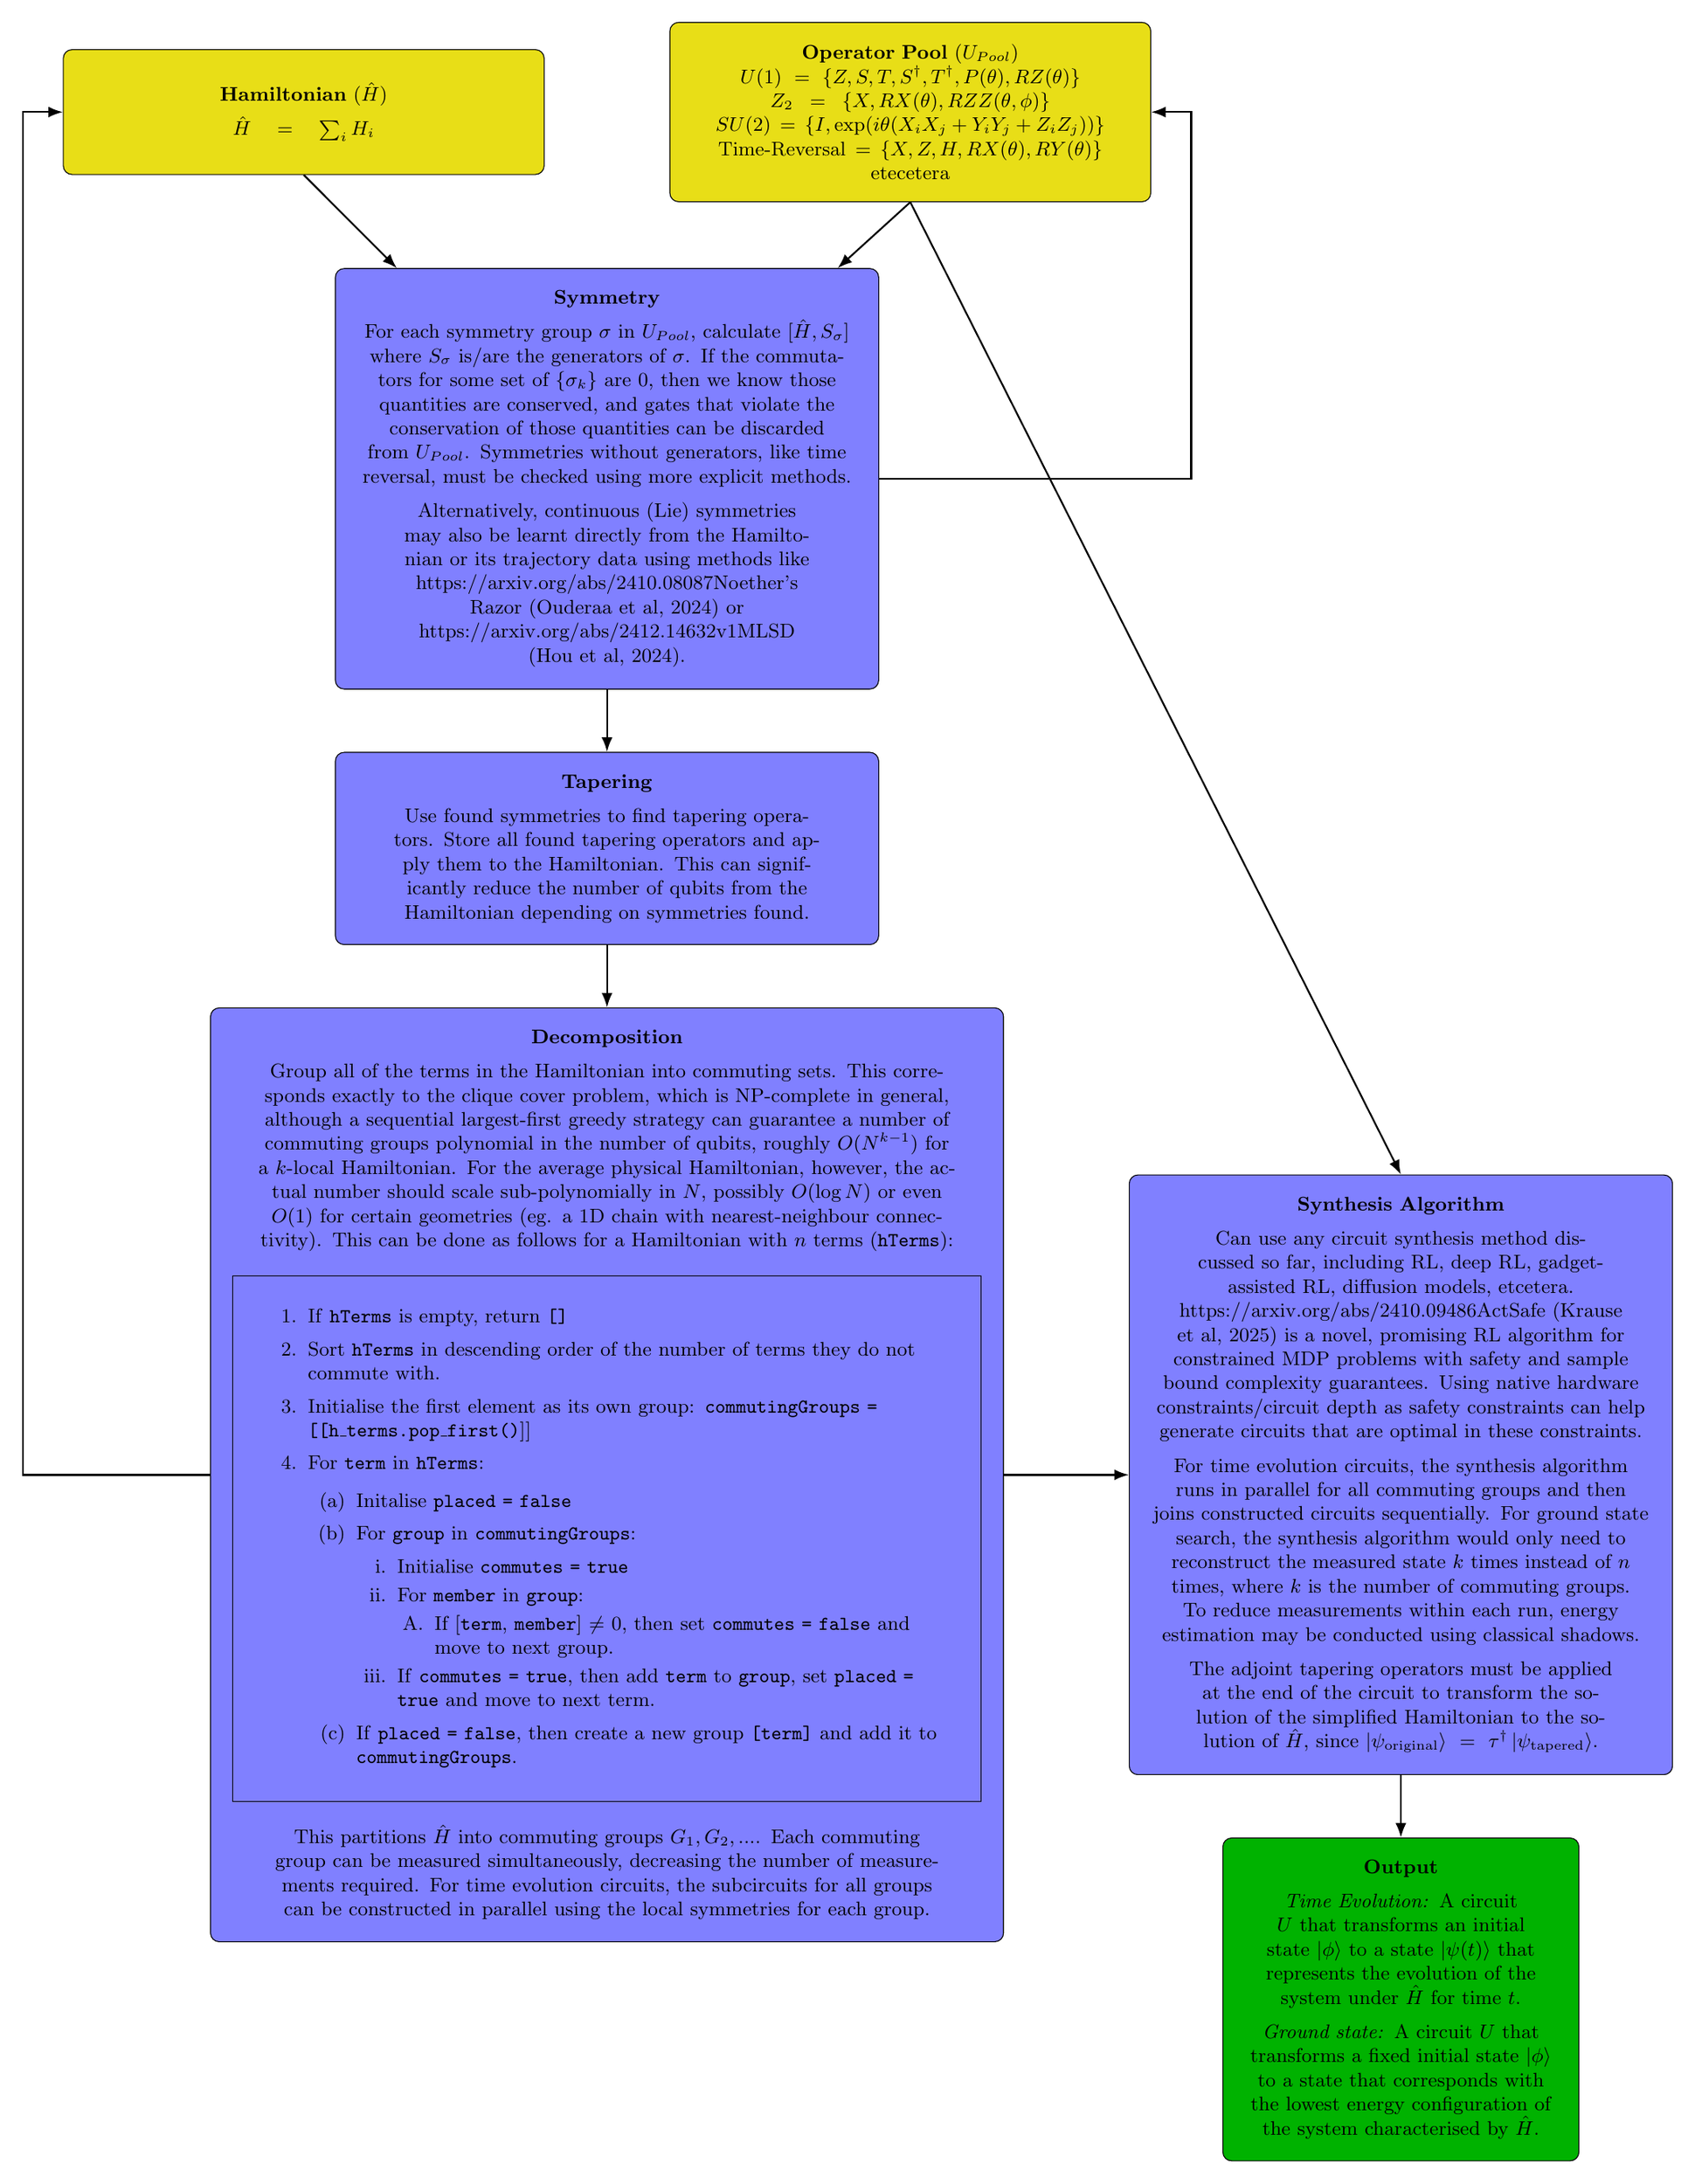
\begin{tikzpicture}[
    input_node/.style={
        draw,
        fill=yellow!90!black, % Dark-ish yellow
        rounded corners,
        text width=7cm,
        align=center,
        inner sep=10pt,
        font=\small,
        minimum height=2cm
    },
    processing_node/.style={
        draw,
        fill=blue!50, % Blue color
        rounded corners,
        text width=8cm,
        align=center,
        inner sep=10pt,
        font=\small,
        minimum height=2cm
    },
    processing_node_decomposition/.style={
        draw,
        fill=blue!50, % Blue color
        rounded corners,
        text width=12cm,
        align=center,
        inner sep=10pt,
        font=\small,
        minimum height=2cm
    },
    label_node/.style={
        font=\bfseries\large,
        align=center
    },
    arrow/.style={
        -Latex,
        thick
    },
    output_node/.style={
        draw,
        fill=green!70!black,
        rounded corners,
        text width=5cm,
        align=center,
        inner sep=10pt,
        font=\small,
        minimum height=2cm
    },
]

% Hamiltonian Node
\node[input_node] (hamiltonian) {
    \textbf{Hamiltonian} ($\hat{H}$) \\
    \vspace{0.5em}
    $\hat{H} = \sum_iH_i$\\
    \vspace{0.5em}
};

% Operator Pool Node
\node[input_node, right=2cm of hamiltonian] (operator_pool) {
    \textbf{Operator Pool} ($U_{Pool}$) \\
    $U(1) = \{Z, S, T, S^\dagger, T^\dagger, P(\theta), RZ(\theta)\}$\\
    $Z_2 = \{X, RX(\theta), RZZ(\theta, \phi)\}$\\
    $SU(2) = \{I, \exp(i \theta(X_i X_j + Y_iY_j + Z_iZ_j))\}$\\
    $\text{Time-Reversal} = \{X, Z, H, RX(\theta), RY(\theta)\}$\\
    etecetera
};

% Symmetry Check Node
\node[processing_node, below=2.5cm of $(hamiltonian)!0.5!(operator_pool)$] (symmetry_check) {
    \textbf{Symmetry} \\
    \vspace{0.5em}
    For each symmetry group $\sigma$ in $U_{Pool}$, calculate $[\hat{H},S_\sigma]$ where $S_\sigma$ is/are the generators of $\sigma$. If the commutators for some set of $\{\sigma_k\}$ are 0, then we know those quantities are conserved, and gates that violate the conservation of those quantities can be discarded from $U_{Pool}$. Symmetries without generators, like time reversal, must be checked using more explicit methods.\\
    \vspace{0.5em}
    Alternatively, continuous (Lie) symmetries may also be learnt directly from the Hamiltonian or its trajectory data using methods like \href{https://arxiv.org/abs/2410.08087}{Noether's Razor} (Ouderaa et al, 2024) or \href{https://arxiv.org/abs/2412.14632v1}{MLSD} (Hou et al, 2024).
};

% Tapering node
\node[processing_node, below= 1cm of symmetry_check](tapering) {
    \textbf{Tapering} \\
    \vspace{0.5em}
    Use found symmetries to find tapering operators. Store all found tapering operators and apply them to the Hamiltonian. This can significantly reduce the number of qubits from the Hamiltonian depending on symmetries found.
};

% Decomposition
\node[processing_node_decomposition, below=1cm of tapering] (decomposition) {
    \textbf{Decomposition} \\
    \vspace{0.5em}
    Group all of the terms in the Hamiltonian into commuting sets. This corresponds exactly to the clique cover problem, which is NP-complete in general, although a sequential largest-first greedy strategy can guarantee a number of commuting groups polynomial in the number of qubits, roughly $O(N^{k-1})$ for a $k$-local Hamiltonian. For the average physical Hamiltonian, however, the actual number should scale sub-polynomially in $N$, possibly $O(\log N)$ or even $O(1)$ for certain geometries (eg. a 1D chain with nearest-neighbour connectivity).
    This can be done as follows for a Hamiltonian with $n$ terms (\hterms):
    \begin{framed}        
    \begin{enumerate}
        \item If \hterms~is empty, return \code{[]}
        \item Sort \hterms~in descending order of the number of terms they do not commute with.
        \item Initialise the first element as its own group: \code{commutingGroups = [[h\_terms.pop\_first()}]]
        \item For \code{term} in \hterms:
        \begin{enumerate}
            \item Initalise \code{placed = false}
            \item For \code{group} in \code{commutingGroups}:
            \begin{enumerate}
                \item Initialise \code{commutes = true}
                \item For \code{member} in \code{group}:
                \begin{enumerate}
                    \item If [\code{term}, \code{member}] $\ne$ 0, then set \code{commutes = false} and move to next group.
                \end{enumerate}
                \item If \code{commutes = true}, then add \code{term} to \code{group}, set \code{placed = true} and move to next term.
            \end{enumerate}
            \item If \code{placed = false}, then create a new group \code{[term]} and add it to \code{commutingGroups}.
        \end{enumerate}
    \end{enumerate}
    \end{framed}
    This partitions $\hat{H}$ into commuting groups $G_1, G_2, ...$. Each commuting group can be measured simultaneously, decreasing the number of measurements required. For time evolution circuits, the subcircuits for all groups can be constructed in parallel using the local symmetries for each group.
};

\node[processing_node, right=2cm of decomposition] (synthesis) {
    \textbf{Synthesis Algorithm} \\
    \vspace{0.5em}
    Can use any circuit synthesis method discussed so far, including RL, deep RL, gadget-assisted RL, diffusion models, etcetera. \href{https://arxiv.org/abs/2410.09486}{ActSafe} (Krause et al, 2025) is a novel, promising RL algorithm for constrained MDP problems with safety and sample bound complexity guarantees. Using native hardware constraints/circuit depth as safety constraints can help generate circuits that are optimal in these constraints.
    \\
    \vspace{0.5em}
    For time evolution circuits, the synthesis algorithm runs in parallel for all commuting groups and then joins constructed circuits sequentially. For ground state search, the synthesis algorithm would only need to reconstruct the measured state $k$ times instead of $n$ times, where $k$ is the number of commuting groups. To reduce measurements within each run, energy estimation may be conducted using classical shadows.\\
    \vspace{0.5em}
    The adjoint tapering operators must be applied at the end of the circuit to transform the solution of the simplified Hamiltonian to the solution of $\hat{H}$, since $\ket{\psi_{\text{original}}} = \tau^\dagger\ket{\psi_{\text{tapered}}}$.
};

\node[output_node, below = 1cm of synthesis](output) {
    \textbf{Output} \\
    \vspace{0.5em}
    \textit{Time Evolution:} A circuit $U$ that transforms an initial state $\ket{\phi}$ to a state $\ket{\psi(t)}$ that represents the evolution of the system under $\hat{H}$ for time $t$.\\
    \vspace{0.5em}
    \textit{Ground state:} A circuit $U$ that transforms a fixed initial state $\ket{\phi}$ to a state that corresponds with the lowest energy configuration of the system characterised by $\hat{H}$.
};

% Arrows
\draw[arrow] (hamiltonian.south) -- (symmetry_check);
\draw[arrow] (operator_pool.south) -- (symmetry_check);
\draw[arrow] (symmetry_check.east) -- ++(5,0) |- (operator_pool.east);
\draw[arrow] (symmetry_check.south) -- (tapering.north);
\draw[arrow] (tapering.south) -- (decomposition.north);
\draw[arrow] (decomposition.west) -- ++(-3, 0) |- (hamiltonian.west);
\draw[arrow] (decomposition.east) -- (synthesis.west);
\draw[arrow] (operator_pool.south) -- (synthesis.north);
\draw[arrow] (synthesis.south) -- (output.north);

\end{tikzpicture}
}

\section{Symmetries}

\subsection{Definitions}

\subsubsection{Commutator}
\begin{definition}{Commutator}{comm_def}
The commutator of two operators $A, B$ is defined as follows:

$$[A, B] = AB - BA$$

When $[A, B] = 0$, or equivalently, $AB = BA$, the operators $A, B$ are said to commute. \cite{cantwell2016introduction}
\cite{vonNeumann:2018:MFQ}

\end{definition}
\begin{itemize}
    \item Given some set of observables $\mathcal{A}, \mathcal{B},...$ and their corresponding operators $A, B, ...$, the commutativity of $A, B, ...$ is \textbf{necessary and sufficient} for the simultaneous measurement of $\mathcal{A}, \mathcal{B},...$ \cite{vonNeumann:2018:MFQ}.

    \item Given a state consisting of $n$ qubits $\ket{\psi} = \bigotimes_{i = 1}^n\ket{\psi_i}$, two spin operators (such as Pauli operators) $I \otimes ...\otimes \sigma^a_j \otimes ... \otimes I$, $I \otimes ...\otimes \sigma^b_k \otimes ... \otimes I$ acting on distinct qubits $a, b$ commute, since the operators act on different factors of the tensor product $\ket{\psi}$ \cite{corry2017symmetry}.
\end{itemize}

\subsubsection{Symmetry}

Let $X$ be a mathematical object. A symmetry transformation is a mapping $g: X \mapsto X$ that preserves a relevant property of $X$, ie. that property is invariant to $g$. The set of all transformations that preserve this property forms a \textit{group} \cite{cantwell2016introduction}. According to Wigner's theorem, transformations on Hamiltonians that preserve transition probabilities must be unitary or anti-unitary operators \cite{corry2017symmetry}.

An operator $U$ is a symmetry of Hamiltonian $\hamiltonian$ if it leaves the Hamiltonian invariant, ie. $U\hamiltonian U^\dagger =\hamiltonian$, which is equivalent to the commutation relation $[\hamiltonian, U] = 0$. \cite{corry2017symmetry}.

\textbf{Discrete Symmetries} are described by discrete groups with finite or countably infinite elements. Some examples of these in quantum mechanics include parity (invariance under spatial inversion), time reversal (invariance under time reversal), etcetera.

\textbf{Continuous Symmetries} are described by a Lie group. Any element $U$ of a one-parameter Lie group can be written in terms of a generator $G$ for a continuous parameter $\alpha$: $$U(\alpha) = \exp\left(\frac{i}{\hslash}\alpha G\right)$$.

If $[\hamiltonian, G] = 0$, then the physical quantity represented by $G$ is a \textit{conserved quantity} \ref{def:cq_def}. This is a quantum mechanical statement of Noether's theorem \cite{ouderaaNoethersRazorLearning2024}. An example of this in quantum mechanics is $SO(2)$.\\

\begin{definition}{Conserved Quantity}{cq_def}
If $O$ is a time-independent observable, then $\hamiltonian(t)$ for all times $t$, then for any initial state $\psi$, the expectation value $\braket{O}_{\psi_t}$ is a \textit{conserved quantity} for the dynamics specified by $\hamiltonian(t)$.

If $\psi$ is an eigenstate for $O$ such that $O\ket{\psi} = \lambda \ket{\psi}$, then $\psi_t$ is an eigenstate for $O$ with the same eigenvalue $\lambda$ \cite{corry2017symmetry}.
\end{definition}

\textbf{Consequences}
\begin{itemize}
    \item If a symmetry operator $U$ does not explictly depend on time, and $[\hamiltonian, U] = 0$, then the expectation value of any observable $A$ associated with $U$ is conserved.
    \item If $\ket{\psi}$ is an eigenstate of $\hamiltonian$ with eigenvalue $\lambda$, then the state $U\ket{\psi}$ ($U$ is a symmetry operator) is also an eigenstate of $\hamiltonian$ with the same eigenvalue $\lambda$.
\end{itemize}

\textbf{Symmetry Preservation in Operators}
If an operator $U$ commutes with a symmetry operator $S$ (ie. $[S, U] = 0$) for a Hamiltonian $\hamiltonian$, then $U$ preserves the $[\hamiltonian, S]$ commutation relation when applied to a state $\ket{\psi}$ evolving under $\hamiltonian$, ie. it preserves the symmetry. More precisely, if a state $\ket{\psi}$ is an eigenstate of the symmetry operator $S$ with the eigenvalue $s$, then the new state $\ket{\psi'} = U\ket{\psi}$ is also an eigenstate of $S$ with the same eigenvalue. This is true because: $$S\ket{\psi'} = S(U\ket{\psi}) = U(S\ket{\psi}) = U(s(\ket{\psi})) = s(U\ket{\psi}) = s\ket{\psi'}$$
\vspace{0.1ex}

\begin{definition}{Twirling Operator}{tw_def}
    Let $U_s$ be a unitary representation of a symmetry group $\sym$. \begin{equation}\twirl{U}{X} = \begin{cases}\begin{aligned}
        \frac{1}{|S|}\sum_{s \in \sym}U_sXU_s^\dagger & ~~~~\sym \text{ is a discrete group}\\
        \int U_sXU_s^\dagger \dd{\mu} & ~~~~ \sym \text{ is a Lie (continuous) group with Haar measure $\mu$}
        \end{aligned}
    \end{cases}\end{equation}
    defines a projector onto the set of operators commuting with all elements of the representation.\cite{meyerExploitingSymmetryVariational2023}
    To prove this, it suffices to show that $[\twirl{U}{X}, U_s] = 0 ~\forall~ X, s \in \sym$, or $U_s \twirl{U}{X}U_s = \twirl{U}{X}$. 
    \begin{equation}
    \begin{split}
        U_s\twirl{U}{X}U_S^\dagger &= U_s\left(\frac{1}{|S|}\sum_{t \in \sym}U_tXU_t^\dagger\right)U_s^\dagger\\
        &= \frac{1}{|S|}\sum_{t \in \sym}U_{st}XU_{st}^\dagger ~~\text{[By the group property $U_sU_t = U_{st}$]}\\
        &= \frac{1}{|S|}\sum_{r \in \sym}U_{r}XU_{r}^\dagger ~~\text{[Relabel $st$ as $r$ (bijective relabeling)]}\\
        &= \twirl{U}{X} ~~~\qed
    \end{split}
    \end{equation}
    
\end{definition}

\textbf{Symmetrising Generators} If an operator $X$ is generated by a generator $G$ from a generator set $\genset$ such that $X = \exp(-i\theta G)$, and $\sym$ is a symmetry with unitary representation $U_s$, then $X'$ generated by $G' = \twirl{U}{G}$ commutes with $U$, ie. \begin{equation}
    [\exp\left(-i \theta \twirl{U}{G}\right), U_s]= 0 ~ \forall ~ G \in \genset, s \in \sym
\end{equation}.

Therefore, given a set of generators $\genset$, a gateset constructed as $\mathcal{X} = \{\exp\left(-i\theta\twirl{U}{G}\right)\ | G \in \genset \}$ is equivariant over symmetry $\sym$ represented by a unitary $U_s, ~s \in \sym$.\cite{meyerExploitingSymmetryVariational2023}

\subsection{Common Symmetries}

\todo{List common symmetries in physical systems and define them}

$U(2), Z_2, SU(2), TRI$

\section{Grouping}
\todo{Show proof for largest-first greedy search guarantees}

\printbibliography
\end{document}
